\section{Linear, ridge and lasso regression}
In this chapter, we implemented linear models: linear regression and ridge regression.
\subsection{Final preprocessing}
Before fitting the linear regression model, it is crucial to preprocess the data. As a consequence, we use the preprocessed dataset prepared earlier.
First and foremost, we have to prepare the sets. We have first to separate the features columns from the target. Then, we split the data into 2 subsets: one for the training and one for the test. We will use later cross-validation on the train dataset.
\begin{lstlisting}[language=python]
X = dataset.loc[:,dataset.columns != 'total_passengers_2022']
y = dataset['total_passengers_2022']
X_train, X_test, y_train, y_test = train_test_split(X, y, test_size=0.33, random_state=42)
\end{lstlisting}

\subsection{Model Implementation and Justification}
The implementation of the linear regression model can be efficiently handled using the \code{scikit-learn} library. The \code{Pipeline} and \code{ColumnTransformer} classes facilitate seamless preprocessing and model training.

\subsubsection{Pipeline and ColumnTransformer}
As the linear regression model only require numerical fields, we need a final preprocessing step to convert any categorical data to numerical one. We chose to use \href{https://scikit-learn.org/stable/modules/generated/sklearn.preprocessing.OneHotEncoder.html}{One Hot Encoder} to convert a $m$-categorical feature into $m$ binary feature.
The \code{ColumnTransformer} allows us to apply different preprocessing steps to numerical and categorical features within a single pipeline. This modularity ensures that each type of data receives the appropriate transformations.

\begin{lstlisting}[language=Python]
preprocessor = ColumnTransformer(
    transformers=[
        ('num', StandardScaler(), num_features),
        ('cat', OneHotEncoder(), cat_features)
    ])
\end{lstlisting}

We use the \code{Pipeline} class to chain the preprocessing steps and the linear regression model. This approach enhances code readability and reproducibility.
\begin{lstlisting}
model = Pipeline(steps=[
    ('preprocessor', preprocessor),
    ('regressor', <MODEL>())
])
\end{lstlisting}

This strategy will be used in the following models because it added a more comprehensive way to define a model and simplifies the encoder. We firstly implemented the one hot encoder in the preprocessing part, but we finally moved the steps in each model to be able to test with or without it.

We first implemented very simple model without , just using Scikit Learn \code{LinearRegression} models. To make our model more robust, we then chose to use \textit{Ridge regularization} (to bound the complexity) and cross-validation. We also implement our own model to practice linear algebra manipulation with Python, but we chose to not include in the model comparison.

\subsection{Ridge and Cross validation}
\begin{itemize}
    \item Ridge regression is a regularization technique. It modifies the ordinary least squares method by adding a penalty to the regression coefficients.
    \item We used cross-validation to ensure our linear regression model's results are robust and reliable. This technique helps prevent overfitting by verifying that the model performs consistently across different subsets of the data, providing a more accurate estimate of its generalizability to new, unseen data.
\end{itemize}
The \href{https://scikit-learn.org/stable/modules/generated/sklearn.linear_model.Ridge.html}{documentation} propose several parameters in addition to $\alpha$. For the cross validation, we chose to use directly \code{GridSearchCV} instead of writing imbrication of \code{for} loops to get the best parameters.
\begin{lstlisting}[language=Python]
param_grid = { 'regressor__alpha': [0.1, 1, 10, 100], ...}
grid_search = GridSearchCV(estimator=model, param_grid=param_grid, cv=5)
\end{lstlisting}

\subsection{Results}
We use the helper functions defined in the first chapter to plot some pictures to analyse the perfromances of our model.

\subsubsection{Raw results}
\begin{table}[h]
    \centering
    \begin{tabular}{ccccc}
        \toprule
        Model &  MSE &  MAE & MedianAE & $R^2$ Score \\
        \midrule
        Linear reg. & 4.232e+10 & 54041 & 20135 & 0.968842\\
        Ridge + CV & 4.242e+10 & 51118 & 15273 & 0.968726\\
        Lasso + CV & 4.366e+10 & 52531 & 15043 & 0.967857\\
        \bottomrule
    \end{tabular}
    \caption{Main metrics to compare linear models}
\end{table}
\begin{figure}[h]
    \centering
    \begin{subfigure}[b]{0.3\textwidth}
         \centering
         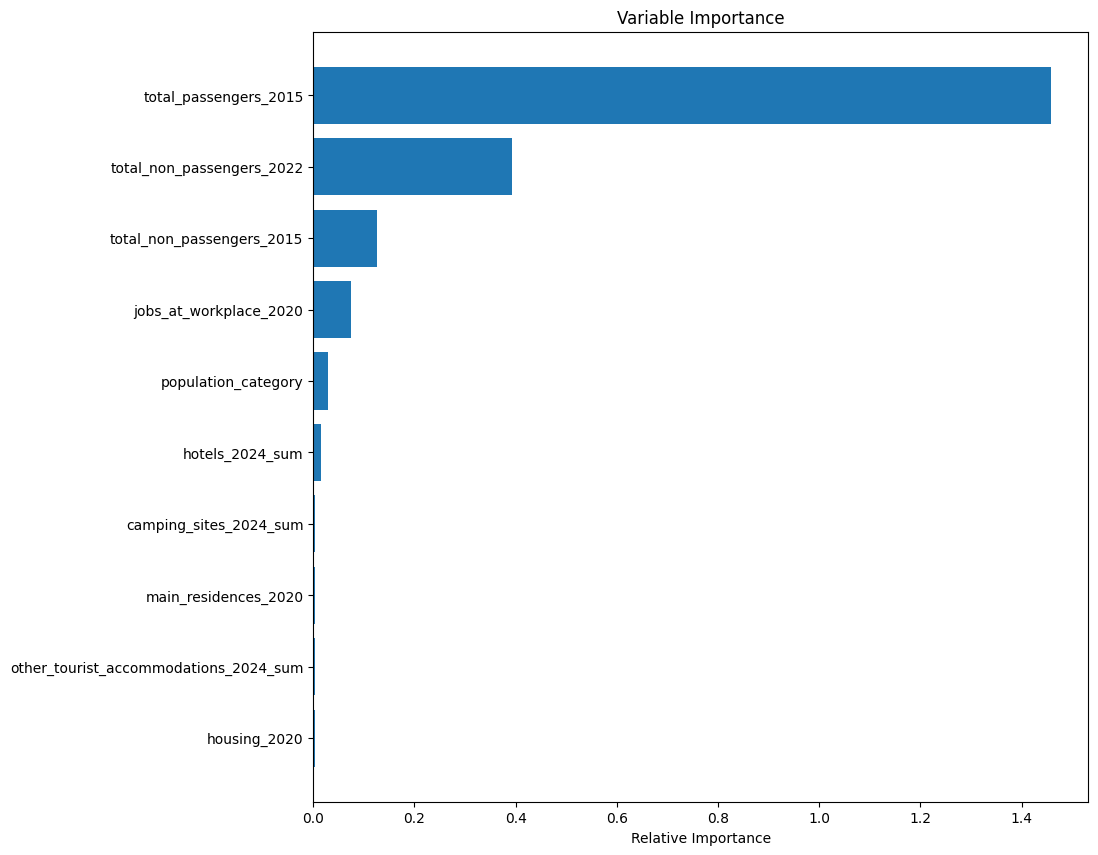
\includegraphics[width=\textwidth]{assets/images/feature-importance-lasso.png}
         \caption{Lasso: Feature importance}
     \end{subfigure}
    \hfill
     \begin{subfigure}[b]{0.3\textwidth}
         \centering
         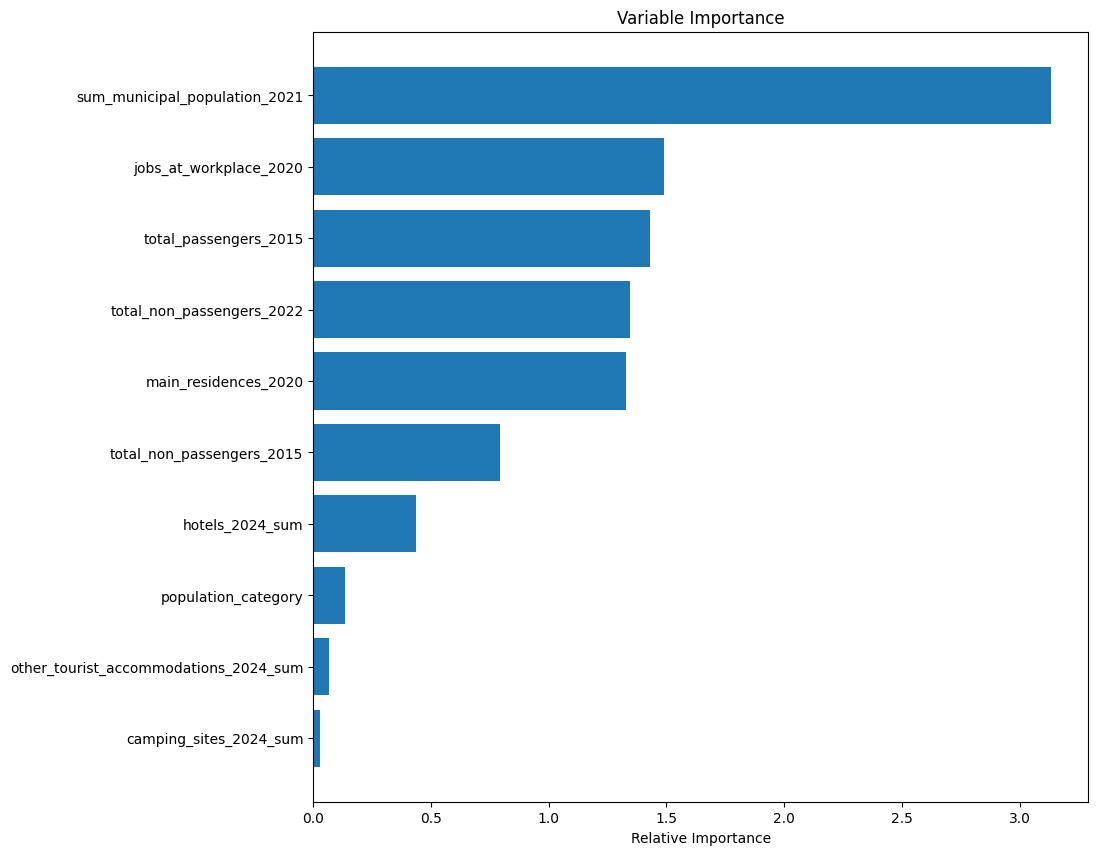
\includegraphics[width=\textwidth]{assets/images/simple-linear-regression-feature-importance.png}
         \caption{Ridge: Feature importance}
     \end{subfigure}
     \hfill
     \begin{subfigure}[b]{0.3\textwidth}
         \centering
         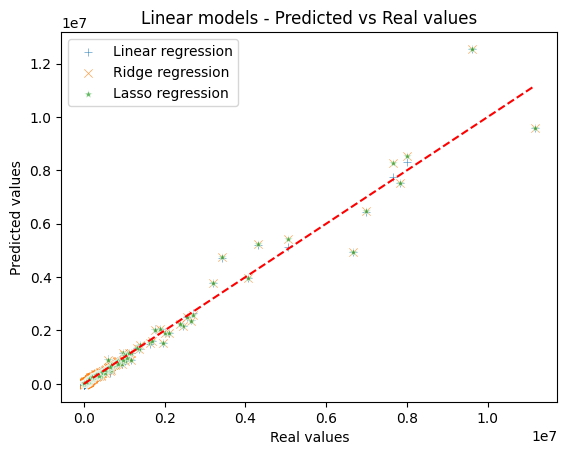
\includegraphics[width=\textwidth]{assets/images/linear-vs-ridge-vs-lasso-prediction.png}
         \caption{Prediction comparison}
     \end{subfigure}
     \caption{Result analysis for linear models}
\end{figure}
In term of metrics presented above, linear regression and ridge regression (+ cross validation) seem to be similar (linear regression is shorter to train). On the other hand, the importance of features is absolutely not the same depending on the model. This is quite unexpected, given that the data provided is the same and the features are normally relatively consistent with the problem set.
\\

It's curious that all points are predicted in the same way by all 3 models, even though they don't take the same features into account at all. The correctness of the models is therefore questionable.


\subsubsection{Interpretation of the results}
Let's analyse a bit the feature importance. We first can see that the two main features are related to localization of the train station, namely the total population living close to this train station and jobs in the attraction area. It is quite logical, but not what we expected. Indeed, it shows the dynamism of the attraction area in term of population (and activity), but we expected to have metrics such as the accomodations available for tourists, the size of the city...